%!TEX root = ../../msc17-game-book.tex


\phChapterWorksheet{Ready, SET, Go!}{Opening Puzzle}

  You'll be faced with quite a few puzzling challenges today, so let's
  start with a quick warm-up! Each team is given a table for their home
  base for this game.

  Your team will begin by collecting game cards from our staff.
  To collect a card, you'll need to answer the arithmetic question
  tossed up by the card's holder. If you're the first person to
  respond with the correct answer, you can take their card back to your
  team's table. Once you've delivered your card, you may then
  attempt to earn more cards.

  \begin{center}
    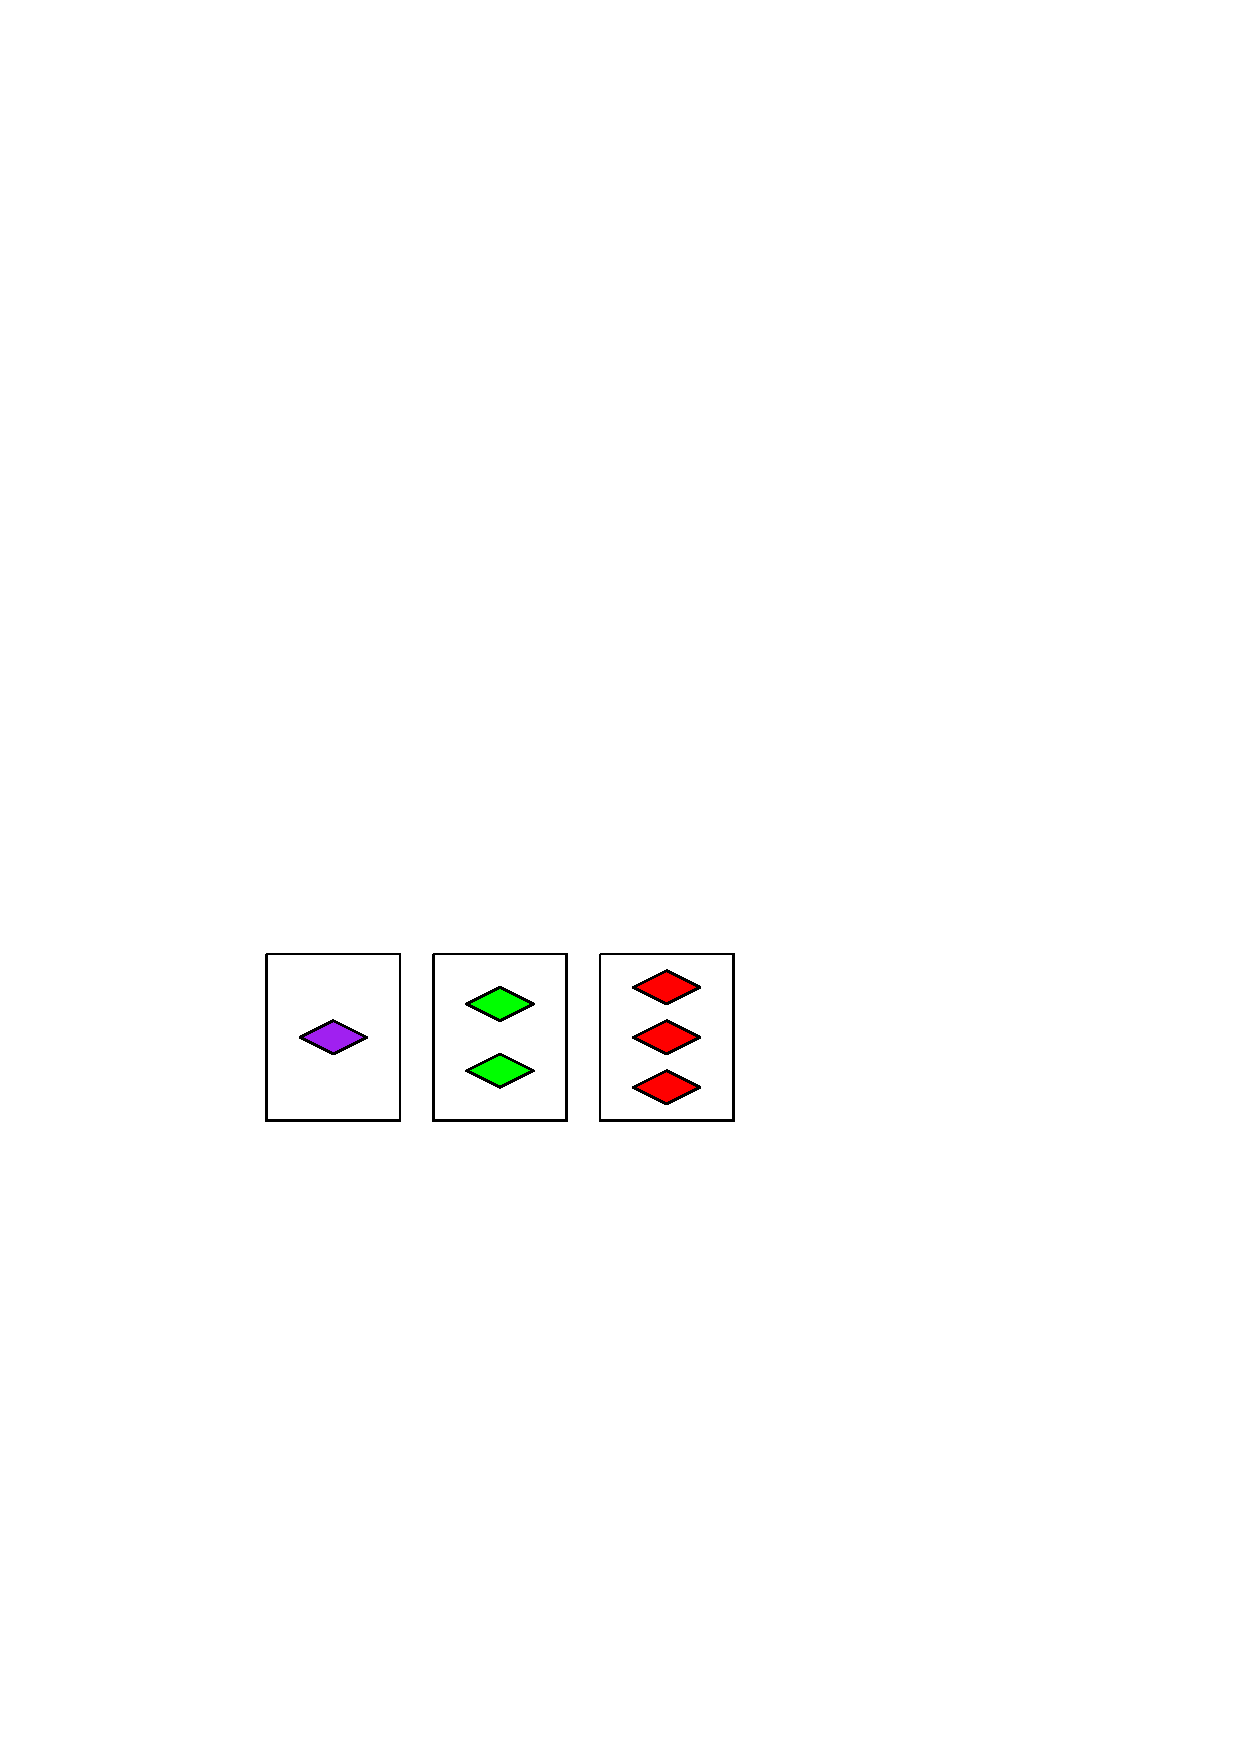
\includegraphics[width=4in]{assets/steven/set-cards.pdf}
  \end{center}

  As your team collects many game cards, you will eventually have
  a three-card SET. Not every combination of three cards forms a SET,
  however... in a SET, each of the following features is either
  \textit{all the same} or \textit{all different}:

  \begin{itemize}
    \item \textbf{Color:}
      \textcolor{red}{red},
      \textcolor{green!60!black}{green}, or
      \textcolor{violet}{purple}.
    \item \textbf{Shape:}
      ovals,
      squiggles, or
      diamonds.
    \item \textbf{Number:}
      one,
      two, or
      three.
    \item \textbf{Shading:}
      empty,
      solid, or
      striped.
  \end{itemize}

  The collection above is a SET because it has all different colors,
  all the same shapes, all different numbers, and all the same shadings.
  After you've found a SET, all of the cards at your table are returned
  to our staff, and you'll start over again.

  \textbf{Once your team has found 5 SETs, you can move on to the
  first round of puzzles.} Good luck!


\phWorksheet{Random Arithmetic}

\begin{multicols}{4}
\begin{itemize}
  \input{etc/random-arithmetic.txt}
\end{itemize}
\end{multicols}
